% PLEASE FILL IN THE PLACEHOLDERS <...>
%
% Diplomarbeit/Studienarbeit/IDP von <NAME>
% Diploma thesis of <NAME>
%
% Title: <TITLE>
%        <TITLE>
%
\documentclass[12pt,a4paper]{report}

%%%%%%%%%%%%%%%%%%%%%%%%%%%%%%%%%%%%%%%%%%%%%%%%%%%%%%%%%%%%

% PACKAGES:

% Define typearea
% a) Use automatic:
\usepackage[BCOR1cm]{typearea}
% b) Or use fixed: 
%\usepackage{geometry}
%\geometry{left=1.5cm,textwidth=18.5cm,top=1.5cm,textheight=26.5cm}

% Use German :
\usepackage[german, USenglish]{babel}
% Use list of tabels, etc. in table of contents:
\usepackage{tocbibind}
% German paragraph skip
\usepackage{parskip}
% Encoder:????
%\usepackage[utf-8]{inputenc}
\usepackage[utf8]{inputenc}
% Use A4-paper efficiently:
\usepackage{a4wide}
% Index-generation
\usepackage{makeidx}
% Einbinden von URLs:
\usepackage{url}
% Include .eps-files (needed also for the LKN-logo):
%\usepackage{epsf}
\usepackage{epsfig}
\usepackage{epstopdf}
% Special \LaTex symbols (e.g. \BibTeX):
\usepackage{doc}
% Include Graphic-files:
%\usepackage{graphics}
% Include Graphic-files:
\usepackage{graphicx}
% Include doc++ generated tex-files:
%\usepackage{docxx}
% Include PDF links
%\usepackage[pdftex, bookmarks=true]{hyperref}
\usepackage{caption}
\usepackage{subcaption}


%%%%%%%%%%%%%%%%%%%%%%%%%%%%%%%%%%%%%%%%%%%%%%%%%%%%%%%%%%%%

% OTHER SETTINGS:

% Pagestyle:
\pagestyle{headings}

% Avoid 'overhang':
\sloppy

% Choose language
\newcommand{\setlang}[1]{\selectlanguage{#1}\nonfrenchspacing}

%%%%%%%%%%%%%%%%%%%%%%%%%%%%%%%%%%%%%%%%%%%%%%%%%%%%%%%%%%%%

% TITLE:

\begin{document}

\thispagestyle{empty}
\newpage

\vspace{5cm}
\begin{center}
    \epsfxsize=4cm
    \epsfbox{figures/LKN_Logo_klein.eps}
\end{center}

\parbox{15cm}{\begin{center} {\sf\bf 
                               \Large  Technische Universität München
                                \smallskip

                               \Large Lehrstuhl für Kommunikationsnetze
                               \smallskip
                              }

                              {\sf \large Prof. Dr.-Ing. Wolfgang Kellerer} 
              \end{center}}  %&

\vspace{4cm}

\begin{center}
        {\bf\Huge Master‘s Thesis} % Studienarbeit, Interdisziplinäres Projekt
\end{center}

\begin{center}
        \settowidth{\baselineskip}{0.4cm}
        {\LARGE 
        Title of the Thesis
        }
\end{center}

\vfill         
{\settowidth{\baselineskip}{0.2cm}
\large\begin{tabular}[l]{ll}
Author: & Last Name, First Name\\
Address: & Somestreet 007\\
         & 12345 City\\
         & Country\\
Matriculation Number: & XXXXXXX\\
Supervisor: & Supervisor Name\\
Begin: & 01. January 1900\\
End: & 01. January 2000
\end{tabular}}

%%%%%%%%%%%%%%%%%%%%%%%%%%%%%%%%%%%%%%%%%%%%%%%%%%%%%%%%%%%%

% MAIN PART:
% Independence and License statements
\thispagestyle{plain}


\vspace*{1cm}
With my signature below, I assert that the work in this thesis has been composed by myself independently and no source materials or aids other than those mentioned in the thesis have been used.



\vspace{2cm}

\hspace{1cm}\begin{tabular}{ccc}
\vspace{-0.3cm}München, 14.10.2016 	&\hspace{4cm} 		& \\
\rule{4.5cm}{0.4pt}					&					&\rule{4.5cm}{0.4pt}\\
Place, Date							&					& Signature			
\end{tabular}

           		






\vspace{4cm}
This work is licensed under the Creative Commons Attribution 3.0 Germany License. To view a copy of the license, visit http://creativecommons.org/licenses/by/3.0/de\\

Or\\

Send a letter to Creative Commons, 171 Second Street, Suite 300, San Francisco, California 94105, USA.

\vspace{2cm}



\hspace{1cm}\begin{tabular}{ccc}
\vspace{-0.3cm}München, 14.10.2016 	&\hspace{4cm} 		& \\
\rule{4.5cm}{0.4pt}					&					&\rule{4.5cm}{0.4pt}\\
Place, Date							&					& Signature	
\end{tabular}
% German abstract:
\setlang{german}
\thispagestyle{plain}

\section*{Kurzfassung} 
A short abstract of the thesis in German. 
% English abstract:
\setlang{USenglish}
\thispagestyle{plain}

\section*{Abstract}
A short abstract of the thesis in English. 



% Table of contents:
\tableofcontents  
% Introduction (Einleitung):
\chapter{Introduction}

One of the most promising directions the field of communication networks has explored in the last years has been the Internet of Things (IoT). An explosion in the capability of everyday objects to connect and communicate with each other via wireless networks promises to mightily expand the boundaries hitherto explored by technology. It also promises to place an almost unmanageable amount of stress into the technologies and infrastructure already in place. 

One of the proposed approaches to ameliorate the overload of connections originating from hundreds of devices to a base station is the grouping of the signals via different algorithms into clusters, which then transmit the aggregated information in one single signal to the rest of the network. 

Although many such algorithms have been proposed, especially coming from the field of Wireless Sensor Networks (WSNs) where data aggregation is much more a matter of course, there has been woefully little attention payed to the viability of such mechanisms in comparison to one another in a scenario conforming to the standards and circumstances of LTE-A and Device to Device (D2D) communication. These kind of considerations are specially relevant when considering the prospective arrival of the IoT, the emergence of concepts such as smart grids and smart cities and the prospect of 5G as the next generation of technology that will have to deal with these issues. 

This thesis aims to do just that: present a coherent and realistic simulation scenario for the clustering of devices within LTE-A, with special attention payed to the interference caused by the simultaneous transmission of information, both within the clusters and between other clusters. This will allow a fair comparison of existing clustering schemes and the degree to which they effectively alleviate congestion in the network.

The main part of the thesis will first present the background of the topic, explaining the difficulties arising from an increase in network-capable devices to the limits posed by the Random Access Procedure in place at the moment. The trade-offs of clustering will be explored, along with an enumeration of some of the most importants algorithms taken into account in this work. This chapter will also give an overview of the factors that need to be contemplated during the simulation of the network, along with the motivation for the choice of the simulation environment. Additionaly, justification will be given for the metrics used for evaluating the results of the clustering algorithms.

Next, the implementations of said simulations will be explored. This chapter will delve deeper into the details of bringing the theoretical models into the code used, with a more in-depth discussion of the decisions taken when finalizing the constraints under which the tests were run. The results that they yield will then be discussed and evaluated in the subsequent chapter, with especial attention payed to a direct comparison of the performance of different clustering algorithms. Finally, a discussion of the results will identify the ones most promising for future research and further development.


% Text Body (Hauptteil)
% Could have multiple chaper-files, e.g.:
\chapter{Background}

\section{Random Access and its Limitations}\label{B:RA}
The necessity of the expansion of the existing standards of wireless networks for the effective handling of large numbers of Machine Type Communications (MTC) had already been identified by the 3GPP early in the implementation of Long Term Evolution (LTE) as a standard in \cite{3rdGenerationPartnershipProject;2011}. As explained in \cite{Laya2014}, a large amount of problems arise with increasingly large amounts of devices connecting to the Base Station (BS) or Evolved Node B (eNodeB) mostly due to the Random Access (RA) procedure that has to be initiated with every connection.

\begin{figure}[!h]
\centering
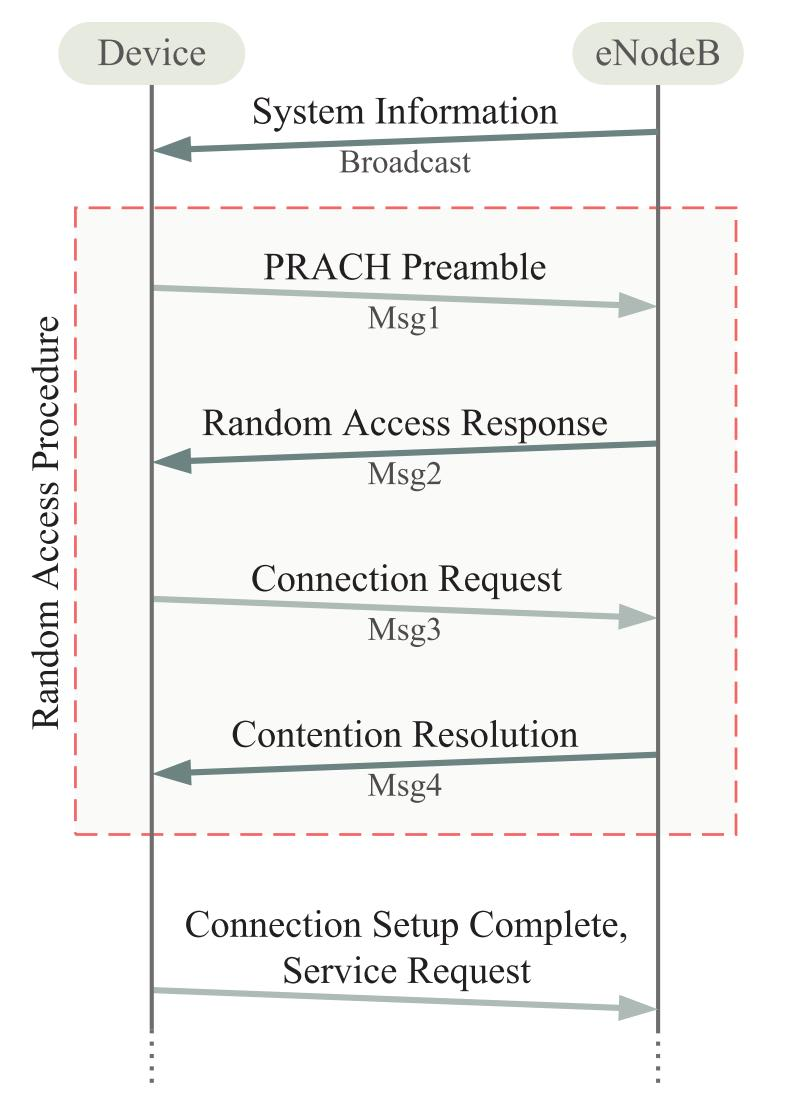
\includegraphics[scale = 0.35]{figures/RACH_LAYA}
\caption{Detail of the Random Access Procedure, \cite{Laya2014}} \label{fig:RACH_LAYA}
\end{figure}

RA procedures occur when a device intends to utilize resources on the Physical Uplink Shared Channel (PUSCH), but has not been given access to the Physical Uplink Control Channel (PUCCH) by the appropriate eNB, which is needed for a scheduling request. As described in \cite{Cox2012}, the User Equipment (UE) then sends a random access preamble to trigger the procedure, in order to gain the desired access, see figure \ref{fig:RACH_LAYA}.

This preamble is chosen randomly from an available set generated with a Zadoff-Chu mathematical sequence and transmitted on the Physical Random Access Channel (PRACH). The eNB then solves any possible collisions that may occur from devices transmitting with the same preamble, granting access to some while ordering others to back off for a certain amount of time. If no access grant is given after several tries, the transmission is considered to have failed.

When a large amount of these connections are initiated in a short time frame, the contention resolution procedures cannot deal with them in a timely manner and many of them are dropped or delayed significantly, waiting for an opportunity to synchronize with the eNodeB, as shown in \cite{Polese2016}. This scenario occurs most often either because the transmission times are highly correlated or just due to the large number of devices in a given area. Both of these circumstances, both in isolation and in conjunction, will be very ordinary occurrences in Internet of Things (IoT) and Smart City applications, concepts speculated to be made possible in the future by Device-to-Device communications. 

\section{Device-to-Device}\label{B:D2D}
One of the technologies that enable the great amount of enthusiasm in the field about the future of interconnected devices is Device-to-Device communication. D2D, as the wireless standard for direct communication between UEs in LTE-A is called, offers a means to expand the existing wireless cellular network to accommodate these type of transmissions. D2D has been widely regarded as one of the technologies heralding a new world of higher interconnectivity and will be a key component in 5G (\cite{6568922}).

D2D communication's potential contributions have been documented widely and continued to be researched to this day. Some of the most popular applications include:
\begin{itemize}
\item Proximity-based services, such as social networking or gaming
\item Public safety and emergency communication applications
\item Local media transmission for businesses or advertisement
\item Vehicle-to-Vehicle communication
\item Localized Peer-to-Peer file transfer
\end{itemize}

In all these applications, D2D presents potential gains in capacity, data rate, latency and load reduction when compared to similar applications that would have to access the network directly before performing their function (\cite{6163598}). This thesis attempts to explore the viability of specific applications of this type of communication as well as quantify some of the aforementioned gains, while taking into account some of the challenges they face, such as interference from other devices.

In this thesis, we work with D2D connections being allocated resources from within the cellular network's bandwidth. These are then kept apart from those used by normal cellular communication after the initial allocation, however. For details on this point, please refer to section \ref{RAP}.

\section{Clustering}\label{B:Cl}

Many approaches have been suggested for the improvement of the circumstances described in section \ref{B:RA}, as summarized succinctly in \cite{Laya2014}, mostly dealing with the improvement of the RA procedures or an expansion of the standards for the Random Access Channel (RACH). Another viable alternative, as presented in a variety of papers (\cite{Wei2012a},\cite{Laya2014a},\cite{Wang2013},\cite{Liao2013}) is the clustering of transmitting devices. This approach aims to reutilize the time and frequency resources within a given set of UEs for different ends, such as decreasing the load on the eNB, increasing the coverage area of the network or minimizing the power consumption of the units involved.

Clustering works by designating devices, called Cluster Heads (CH) that act as relays between the different UEs in a certain area and the eNB or a further Cluster Head by aggregating the data sent to it and relaying it. This aggregation can occur simply by gathering the data over a period of time and transmitting the same information in one long message, as in \cite{Shariatmadari2015}, or through actual elimination of data redundancy, as contemplated in \cite{Riker2015}.

The Cluster Heads themselves are often dedicated gateways, as utilized in \cite{Niyato2011} or \cite{Shariatmadari2015} and have been utilized especially in Wireless Sensor Networks with some frequency. Another, very promising approach to creating clusters is the integration of D2D communication to eliminate the need for dedicated Cluster Heads and enable dynamic cluster forming, depending on the circumstances experienced by the network. This type of clustering scheme promises to bring much needed flexibility to the creation of these structures, since they do not necessitate much investment in additional infrastructure, nor much prior information about the density of devices. D2D communications bring many benefits, both for the user and the network, but also raise several issues that have not been yet properly investigated so far, see \cite{Klugel2014}. As devices utilize the same shared resources in a constrained space, interference becomes more of an issue as devices elect to transmit their messages in the same bandwidth at the same time. This topic of inter-cluster interference due to reuse of resources and its effects on possible D2D connections is of great interest to this thesis. 

\begin{figure}[H]
\centering
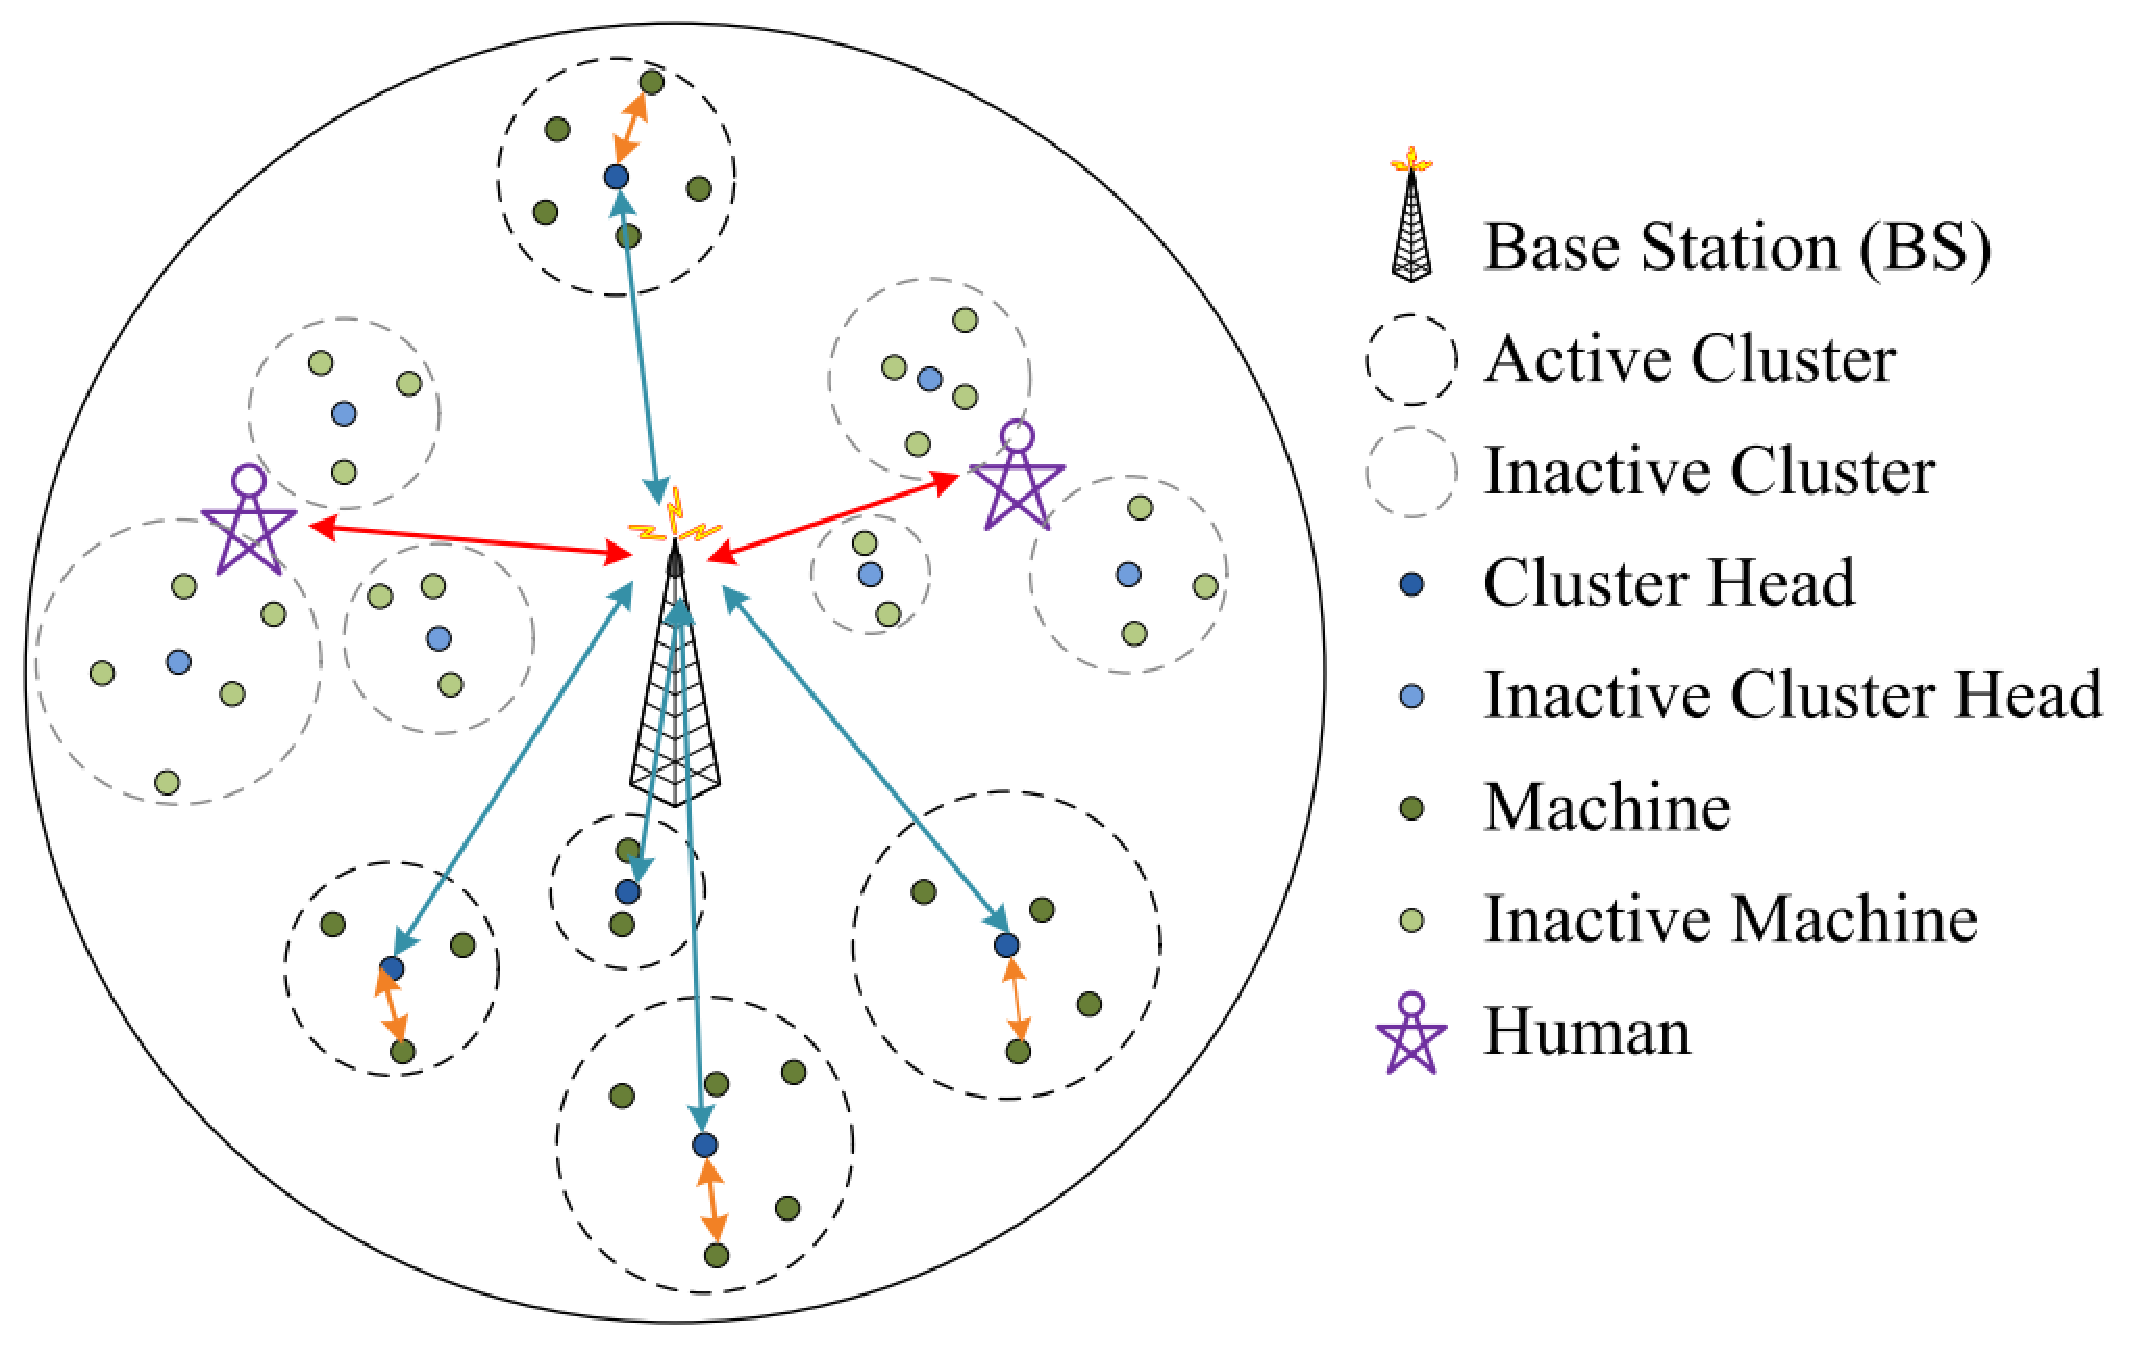
\includegraphics[scale = 0.25]{figures/D2D_clustering}
\caption{Example of D2D Clustering in a network \cite{Wang2013}}
\end{figure}

As mentioned earlier, this sort of application is specially intriguing in the case of highly dense Smart Cities and the IoT. Despite the promising future offered by this technology, there is a dearth of research concerning this specific scenario, be it a comparison of different clustering schemes or even the detailed simulation of one clustering scheme with varying parameters. Although detailed surveys of algorithms exist, such as \cite{Jiang2009} or \cite{Afsar2014}, they mostly center around description and classification. This thesis is meant to alleviate this lack of exploration. Not only will different clustering schemes be analyzed and compared fairly, they will also be scrutinized under different criteria, allowing for an assessment of their viability. This will hopefully give a direction to future possible research in this area, by highlighting some of them as viable or others as not viable at all.


The next chapters will explain in detail the steps taken to create the simulation environment as well as a presentation and evaluation of the results it yielded.
\chapter{Implementation} \label{Implementation}

As mentioned in the preceding chapters, the development of the simulation environment was as much a goal of this thesis as any; we seek to lay the groundwork for further investigation in this field with a credible system that reproduces faithfully the conditions found in a dense, urban environment with many devices capable of accessing the network. Ideally, the work presented here will be refined and will continue to be used on investigations in this area.

For the creation of such a testing environment, five elements were recognized as of utmost importance to the validity of the tests and the author sought to implement them accordingly. In the following, they will be presented with detail, justifying the sources of the models and the parameter choices made.

The aforementioned elements are:

\begin{itemize}
	\item Generation and distribution of UEs %\ref{PPP}
	\item Path loss (attenuation) %\ref{PL}
	\item Shadow fading %\ref{SF}
	\item Random access procedure and interference %\ref{RAP}
  \item Clustering algorithms
\end{itemize}

The actual simulations, as well as the measures used to quantify the relative performance of each algorithm are presented in chapter \ref{Results}.

\section{Generation and distribution of UEs} \label{PPP}
Often called a ``completely'' random process, a Poisson process is a process where every event is stochastically independent of all other points in it, see \cite{Keeler2016}. This generation process is common in investigations about the performance of networks, as eloquently expressed by \cite{Keeler} In our case, the Poisson-distributed random variable are the number of points in the bounded region we are investigating. The distribution is described by the following probability mass function:

\begin{equation} \label{eq:Poisson}
P\left( x\ points\ in\ region \right) = \frac{{e^{ - \lambda } \lambda ^x }}{{x!}}
\end{equation}

By providing the $\lambda$ above, often called mean density (\cite{Keeler2016}), we can adjust the expected amount of points generated in a given area. In order to evaluate the robustness of different algorithms, the tests were made with a variety of $\lambda$ values. The generated amount of points are then distributed in the given area with a uniform distribution, where both the $x$ and $y$ value are distributed along the appropriate axis. In both cases, the \textit{Python} package \textit{NumPy} was utilized for the realization of the random distributions.

\begin{figure}[!h]
\centering
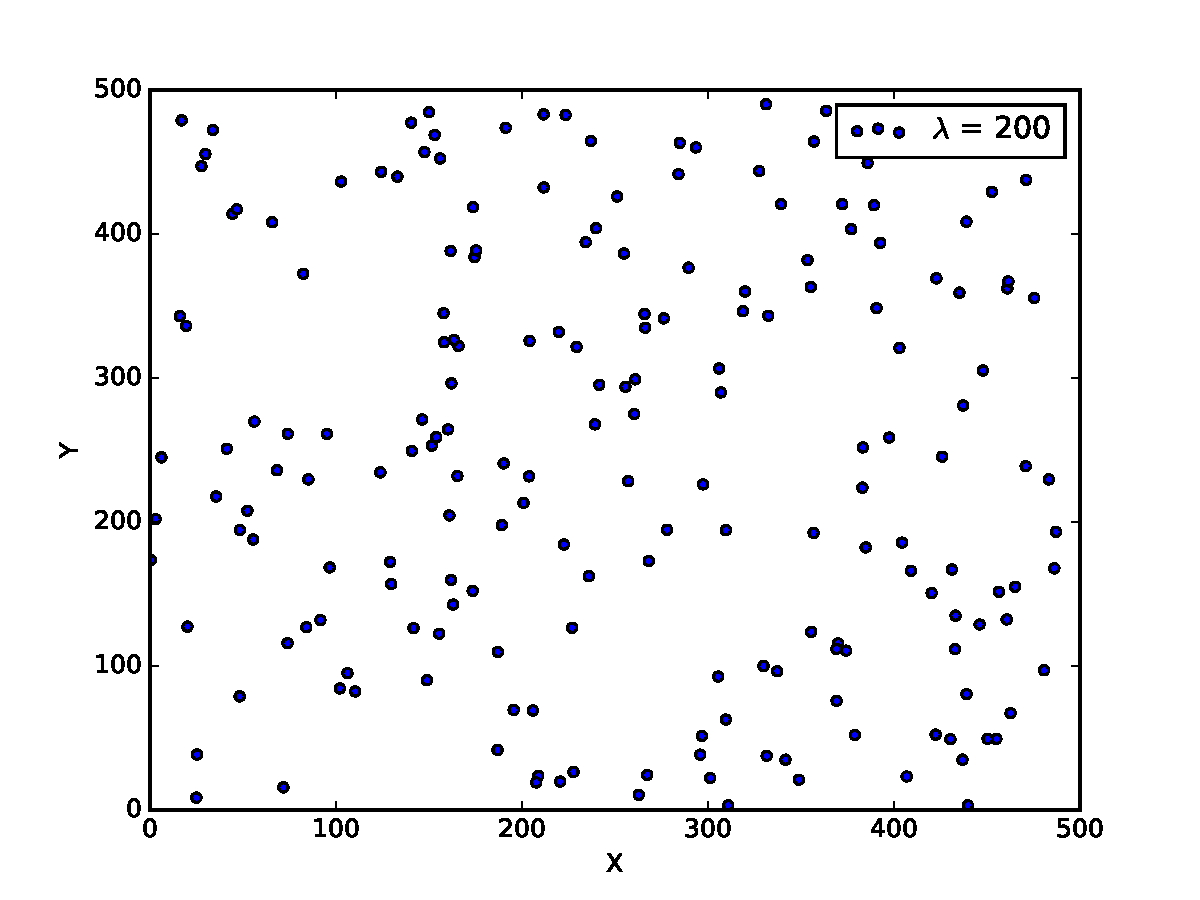
\includegraphics[scale = 0.6]{figures/PPP}
\caption{Example of a PPP with $\lambda = 200$}
\end{figure}

Thus we have generated the number and position of all our UEs according to a Poisson point process (PPP).

\section{Path loss (attenuation)} \label{PL}
Whenever transmission between devices is being investigated, loss due to attenuation as the signal propagates through space is an unavoidable topic. Distance degrades electromagnetic waves in terms of power in any real system and any simulation that does not reflect this phenomenon is simply not valid. 

In search of the best documented and most forward-looking models available, we settled on the use of METIS (Mobile and wireless communications Enablers for the Twenty-twenty Information Society), a EU Project that seeks to promote the definition of 5G mobile technologies. Its channel model, presented in its deliverables (\cite{Raschkowski}) was especially insightful. 

For the purposes of this thesis, the Stochastic Model, a ``geometry-based stochastic channel model'', was chosen for the way it lined up with our own goals, especially when it came to level of detail and complexity. Their figures are based on previous efforts by 3GPP studies to model these same phenomena. Due to the highly dense, urban system we are investigating, propagation scenario number one, ``Urban Micro'' was selected. Due to the constraints of this thesis, we narrowed our focus on Outside-to-Outside (020) connections, although the integration of Outside-to-Inside (O2I) could be a feature of future research.

When calculating the attenuation for a given path between two devices, there emerge two distinct cases, depending on whether there are any significant obstacles between the two of them: Line-of-sight (LOS) and Non-line-of-sight (NLOS).



\subsection{Manhattan grid} \label{mh_grid}
In order to determine whether a given link is a LOS or NLOS link, we need information about the obstacles present in the path between the two. In our case, we don't consider objects like cars and people explicitly, but rather account for all such minor objects and reflections they might create with a stochastic model (see \ref{SF}). Buildings, on the other hand, represent such massive, nigh-impenetrable objects that we must contemplate them concretely.

The preferred method mentioned in the METIS deliverables is the use of a ``Manhattan-like'' grid, meaning a city-layout comprised of rectangular blocks criss-crossed by wide streets. To determine both the size and the overall layout of our Manhattan Grid, we again turn to the extensive work done by METIS. The measurements with which their relevant models were tested were run in Madrid, with a grid of around 500 meters of both length and width. We homogenized the scenario by having exclusively square blocks, but maintained both the street width and the general dimensions. We also fixed the position of the eNodeB exactly at the middle of the grid for those clustering algorithms that needed its position.


\begin{table}[htbp]
\begin{center}
 \begin{tabular}{||p{3cm}|p{3cm}||} 
 \hline
 \textbf{Parameter} & \textbf{Value}\\
 \hline\hline
 Grid Dimensions & 500 m $\times$ 500 m \\ 
 \hline
 Block Width & 110 m \\
 \hline
 Block Length & 110 m \\
 \hline
 Street Width & 20 m \\
 \hline
 eNB position & (250\,\text{m},\,250\,\text{m})\\
 \hline
\end{tabular}
\end{center}
\caption{Manhattan grid parameters}
\end{table}

The introduction of an explicit grid raises the issue of the positioning of our UEs again. Having scattered them in a Poisson point process (see \ref{PPP}), some inevitably now find themselves inside a building and not on the street, as is necessary for our O2O simulations. We overcome this obstacle by simply finding the shortest route from the position inside a block to the street: as the UE position is random, so too is the route taken. Thus we avoid completely discarding the randomness of their positioning. The results can be seen in figure \ref{fig:mh_grid_own} and compared to the actual city grid used for METIS measurements (figure \ref{fig:Madrid}).

\begin{figure}
\centering
\begin{subfigure}{.35\textwidth}
  \centering
  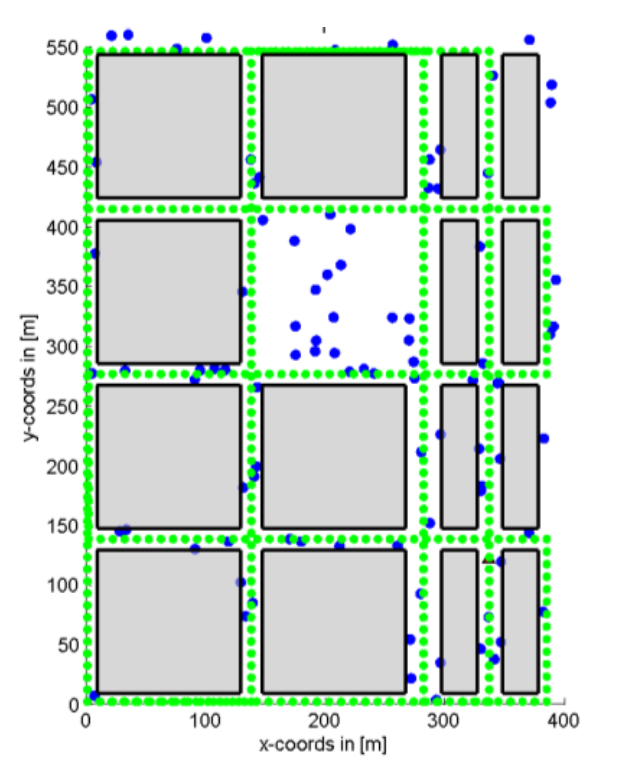
\includegraphics[width=1.2\linewidth]{figures/Madrid}
  \caption{Madrid grid \cite{Raschkowski}}
  \label{fig:Madrid}
\end{subfigure}%
\begin{subfigure}{.65\textwidth}
  \centering
  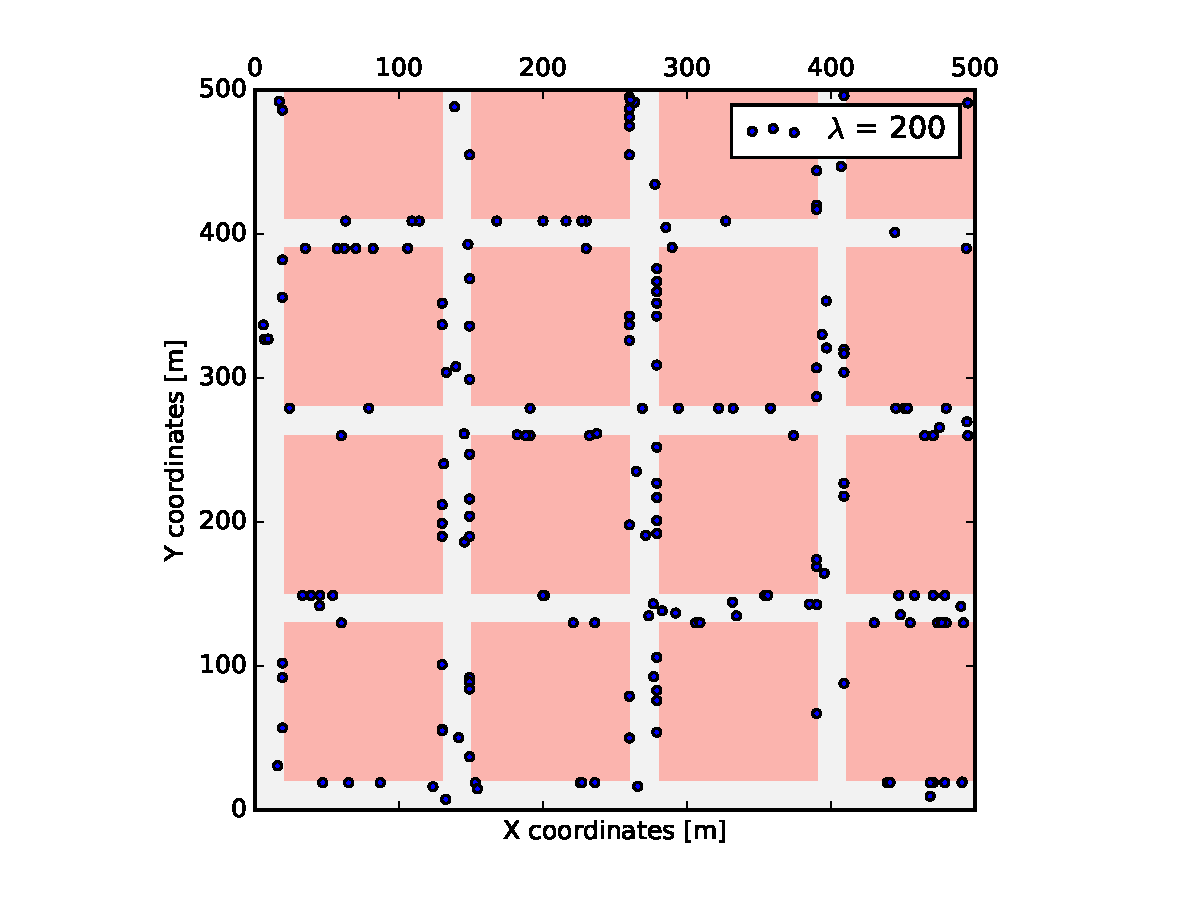
\includegraphics[width=1.058\linewidth]{figures/mh_grid}
  \caption{Own implementation, including moved UEs}
  \label{fig:mh_grid_own}
\end{subfigure}
\caption{Comparison between two Manhattan Grids}
\label{fig:mh_grid}
\end{figure}


With a Manhattan-like layout at the ready, questions about whether a link has LOS or not become much easier to answer.

\subsection{Line-of-sight} \label{LOS}
The overall model for pathloss used by \cite{Raschkowski} is derived specifically from the one presented in \cite{ReportITU-RM.2135-12009} by the ITU (International Telecommunication Union) and covers a wide frequency range (0.8 to 60 GHz). Distances between 10 and 500 meters are thus defined by two distinct equations, depending on whether the distance between the two points is greater than a certain ``breakpoint distance''. The distance $d^\prime_{BP}$ in question is defined by
\begin{equation} \label{eq:dbp}
d^\prime_{BP} = 0.87\, \exp\bigg( -\frac {log_{10} \big( \frac {f_c} {1\,\text{GHz}} \big)} {0.65} \,\bigg)\,\frac{4\,h^\prime_{BS}h^\prime_{UE}}{\lambda_{WL}}\,,
\end{equation}
with $h^\prime_{BS}$ as the effective height of the Base Station and $h^\prime_{UE}$ the effective height of the UE, with ``effective" denoting adjusting for environment height $h_e$. The $\lambda_{WL}$ is the wavelength of the signal, which is calculated from the center frequency $f_c$ and the speed of light $c$. It must be mentioned that for our transmissions, the height of both the origin and destination device will be identical more often than not, due to cluster connections being D2D links.

An additional ``pathloss offset'' $PL_1$ is defined in order to bring the model in agreement with the control measurements performed by METIS and is designed to account for elements like multipath fading.

\begin{equation} \label{eq:PL_1}
PL_{1|dB} = -1.38\,\log_{10}\,\bigg( \frac {f_c}{1\,\text{Ghz}} \bigg) + 3.34
\end{equation}


The actual pathloss equations are given as a function of distance $d$ by

\begin{equation} \label{eq:PL_LOS_1}
  PL_{LOS}(d)_{|dB} = 10\,n_1\,\log_{10}\bigg( \frac{d}{1\,\text{m}} \bigg) + 28.0 + 20 \log_{10} \bigg( \frac{f_c}{1\,\text{GHz}} \bigg) + PL_{1|dB}
\end{equation}
for $10\,\text{m}\,<\,d\, \le \,d^\prime_{BP}$ and
\begin{equation} \label{eq:PL_LOS_2}
  PL_{LOS}(d)_{|dB} = 10\,n_2\,\log_{10}\bigg( \frac{d}{d^\prime_{BP}} \bigg) + PL_{LOS}(d^\prime_{BP})_{|dB}
\end{equation}
for $d^\prime_{BP}\,<\,d\, \le \,500\,\text{m}$ (compare with \cite{Raschkowski}). The parameters $n_1 = 2.2$ and $n_2 = 4.0$ are the power decay constant on both sides of the break point distance.

\subsection{Non-line-of-sight} \label{NLOS}
Most of the connections available to a given UE will be NLOS links. These happen whenever the UE tries to communicate with a device that is not on its same street and thus the signal has to travel a more convoluted way in order to be received. METIS defers explicitly to the final channel models, created by WINNER+ (Wireless World Initiative New Radio+) in \cite{Heino2010}. WINNER+ is a private consortium looking to further develop the IMT-A (International Mobile Telecommunications-Advanced) standards. 

The conceptual NLOS model in itself comes from an even earlier work, \cite{Meinila2009}, which details the relevant parameters for NLOS communication in an urban setting. In these cases, the corners resulting from intersecting streets act as relay nodes for the signal. \cite{Meinila2009} designates two distances needed to calculate the pathloss in this route, see figure \ref{fig:d1_d2}, where $d_1$ is distance from relay node to BS and $d_2$ to the UE. As was the case for the difference in heights between UE and BS, seeing as the links we are investigating are D2D, there is no real clear theoretical distinction between $d_1$ and $d_2$. However, we keep the distinction intact (with the same emitter/receiver relation) owing to the fact that ``[t]hough the pathloss between BS and UE must be the same regardless of the direction of signal transmission due to reciprocity, the pathloss \textit{models} do not necessarily hold the reciprocity'' (\cite{Raschkowski}).

\begin{figure}
\centering
\begin{subfigure}{.5\textwidth}
  \centering
  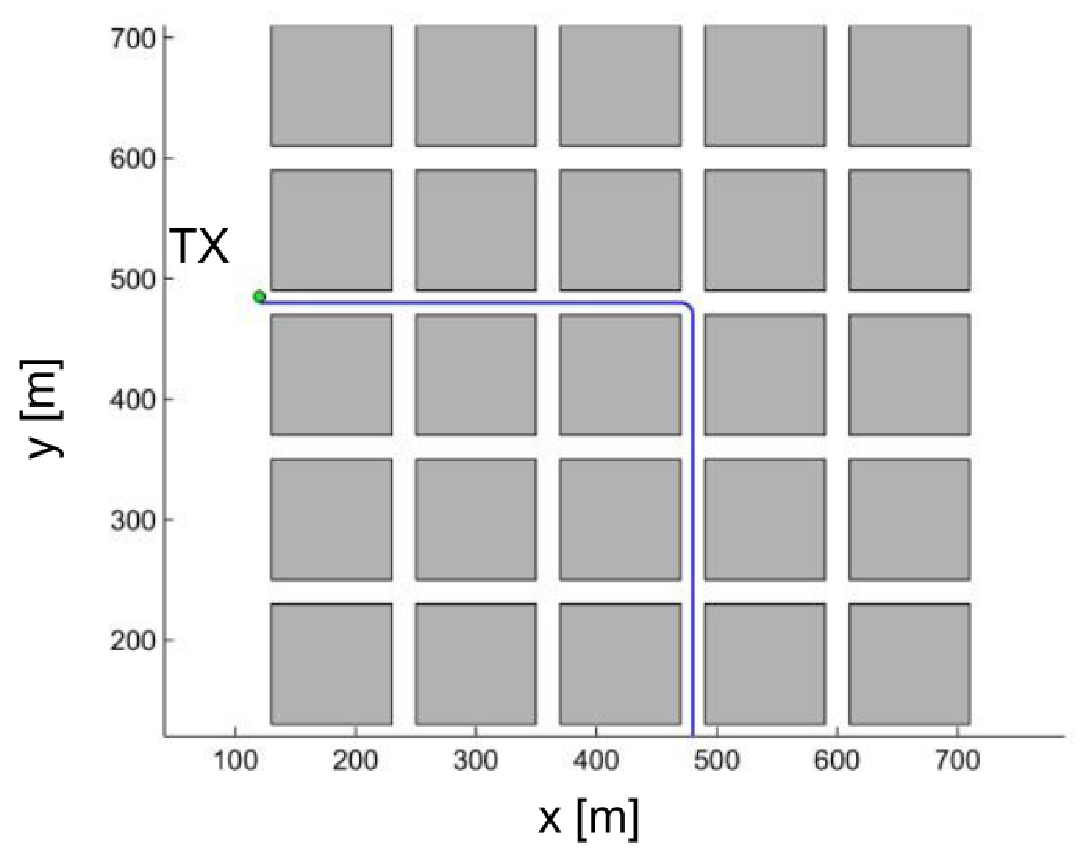
\includegraphics[width=1\linewidth]{figures/node_relay}
  \caption{Node Relay example \cite{Raschkowski}}
  \label{fig:node_relay}
\end{subfigure}%
\begin{subfigure}{.5\textwidth}
  \centering
  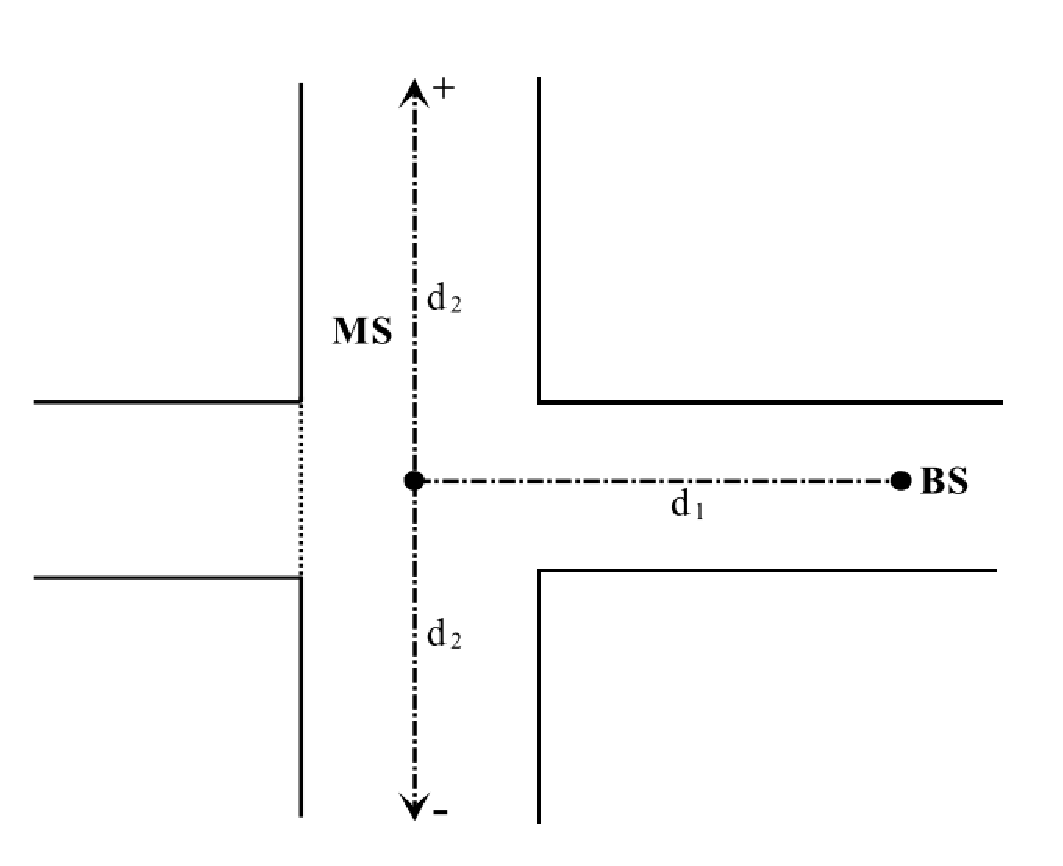
\includegraphics[width=1\linewidth]{figures/d1_d2}
  \caption{Distances $d_1$ and $d_2$ \cite{Meinila2009}}
  \label{fig:d1_d2}
\end{subfigure}
\caption{Calculation of NLOS path}
\label{fig:nlos_path}
\end{figure}

Thus, the formula for pathloss in the studied case is presented in \cite{Raschkowski} after a small simplification and again featuring the ``pathloss offset'' (equation \ref{eq:PL_1}) mentioned in \ref{LOS}:

%\begin{equation} \label{eq:NLOS}
\begin{equation} \label{eq:NLOS}
\begin{split}
  PL_{NLOS}(d_1,d_2)_{|\text{dB}} = & \,PL_{LOS}(d_1)_{|\text{dB}} + 17.9 - 12.5\,n_j \\
  & + 10\,n_j\,\log_{10} \bigg( \frac {d_2} {1 \text{m}} \bigg) + 3 \log_{10} \bigg( \frac { f_c } { 1 \text{GHz} } \bigg) + PL_{1|\text{dB}},
\end{split}
\end{equation}
where $n_j$ is a power decay constant calculated as

\begin{equation} \label{eq:n_j}
n_j = \max (2.8 - 0.0024\,d_1,\,1.84).
\end{equation}

In a rectangular Manhattan grid such as ours, a only two intersections are needed as relays in order to connect any two given points on the grid. An algorithm was thus created to calculate the shortest possible distance between the two devices using a maximum of two intersections. We take the shortest possible route because the signal spreads omni-directionally. An example of a calculated route between two points can be seen in figure \ref{fig:two_points}.

\begin{figure}[H]
\centering
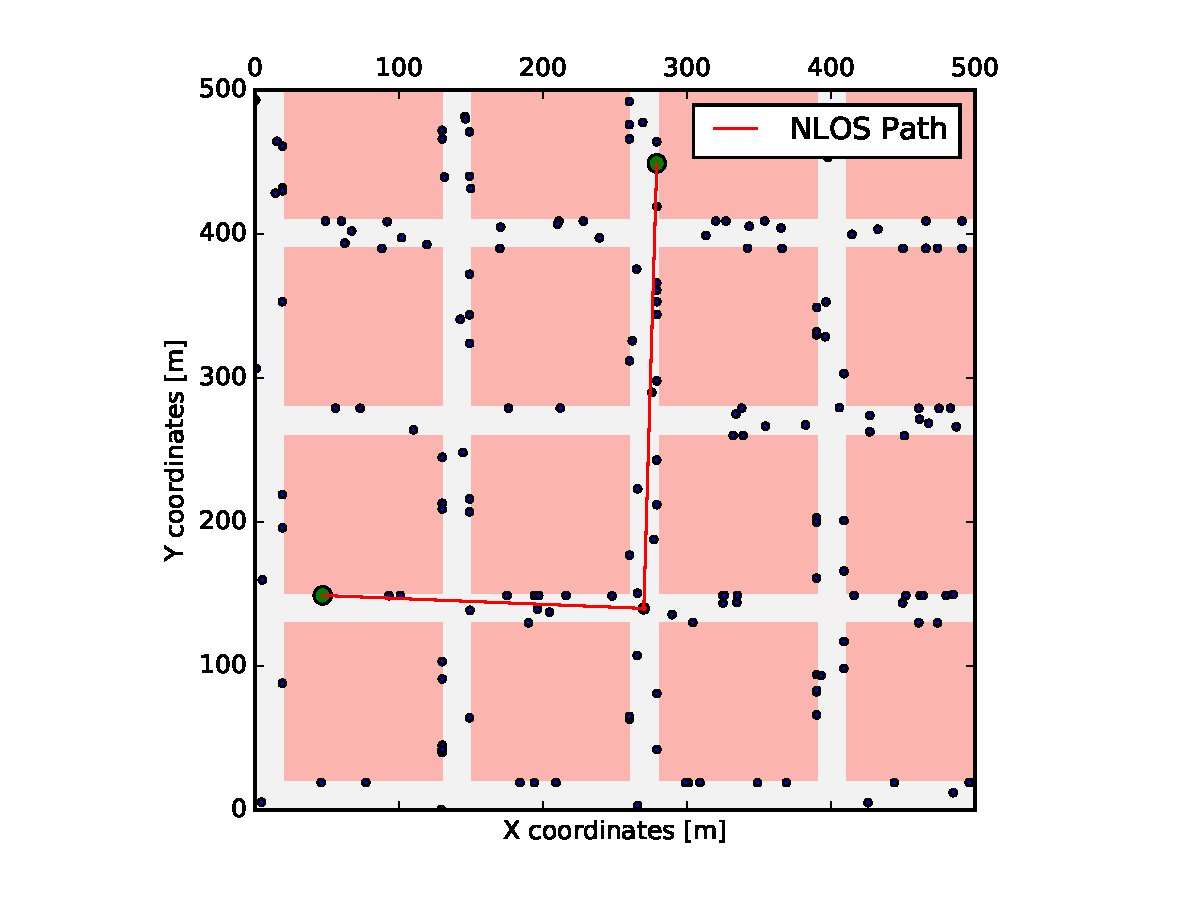
\includegraphics[width=.7\linewidth]{figures/two_points}
\caption{Visualization of NLOS path with intersection acting as relay node}
\label{fig:two_points}
\end{figure}

\section{Shadow fading} \label{SF}
As mentioned in \ref{mh_grid}, Shadow Fading - meaning the effects on the signal caused by smaller obstacles - as well as the reflections they create are modelled through a stochastic model. This type of fluctuation, called ``Shadow Fading'' or ``long-term fading'' is often realized through a Gaussian distribution in the logarithmic scale (also called a log-normal distribution), as asserted in \cite{Forkel2004} and shown below in its probability density function. In our case, we followed METIS specifications and set $\mu_{L_s} = 0$ and $\sigma_{L_s} = 7 \text{dB}$.

\begin{equation} \label{eq:SF}
p(L_s) = \frac{1}{{\sigma_{L_s} \sqrt {2\pi } }}\,\exp\bigg(-\frac{(L_s - \mu_{L_s})^2}{2\,\sigma_{L_s}^2}\bigg)
\end{equation}

While any given point is distributed randomly along the normal distribution, completely random and uncorrelated shadow fading variables make little sense when one considers that the effects of any given set of obstacles won't change much in the space of a couple of meters. In order to account for the necessary correlation that these shadow fading variables experience, a normalized autocorrelation function is introduced, both in \cite{Forkel2004} and \cite{Raschkowski}, with a decorrelation value suggested by METIS $d_{corr} = 8 m$.

\begin{equation} \label{eq:corr}
R(\Delta x) = \exp\bigg(-\frac{|\Delta x|}{d_{corr}}\,\ln(2)\bigg)
\end{equation}

After generating the shadow fading variables with equation \ref{eq:SF} and the autocorrelation coefficients with equation \ref{eq:corr}, both matrices are convoluted to generate the correlated values. Convolution does not alter the underlying distribution, but it does elicit a correction of the mean and standard deviation (compare with \cite{Forkel2004}) in order to return it to the values of the original Gaussian distribution. Our realization is shown below, both before and after the aforementioned correction for spatial correlation.

%\centering
\begin{figure}
\centering
\begin{subfigure}{.5\textwidth}
  \centering
  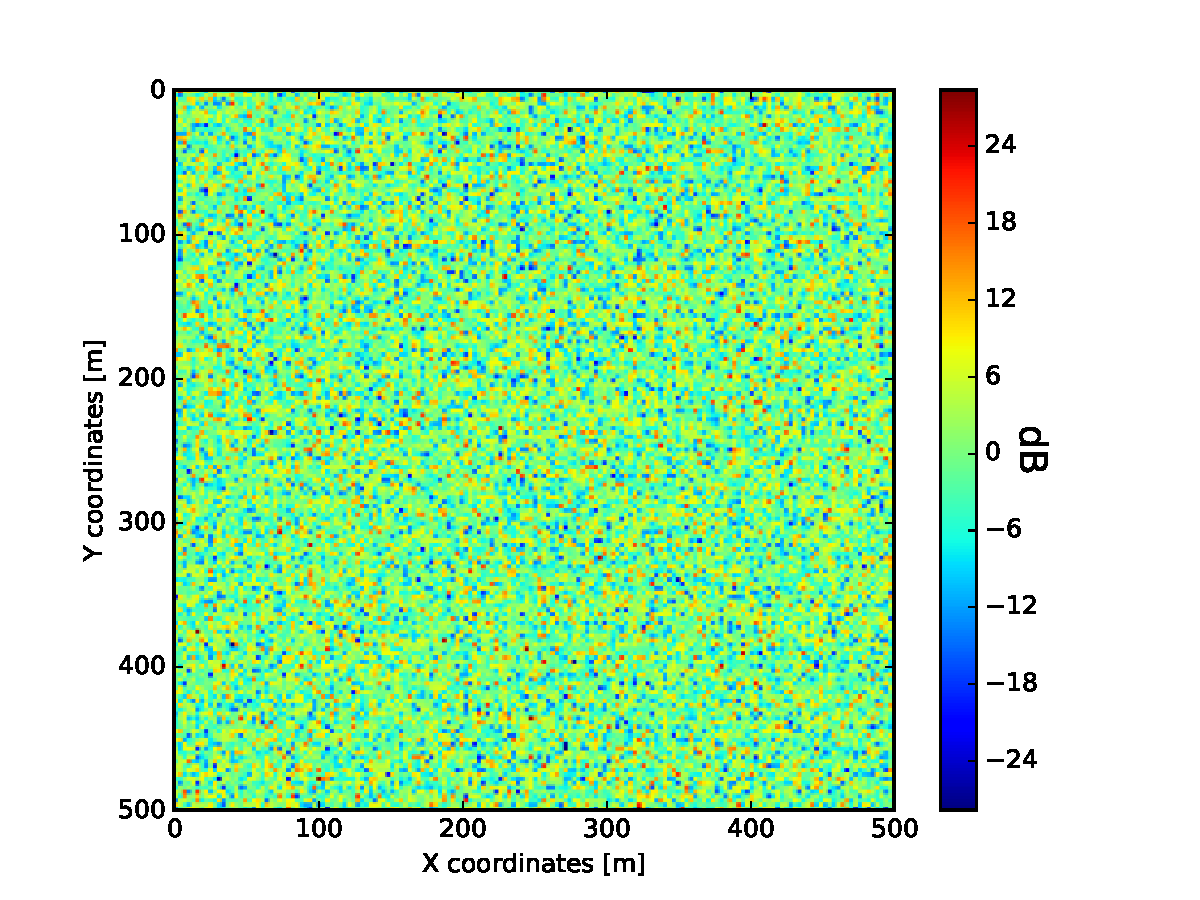
\includegraphics[width=1.1\linewidth]{figures/noise_before}
  \caption{Uncorrelated Shadow Fading values}
  \label{fig:sf_no_correlation}
\end{subfigure}%
\begin{subfigure}{.5\textwidth}
  \centering
  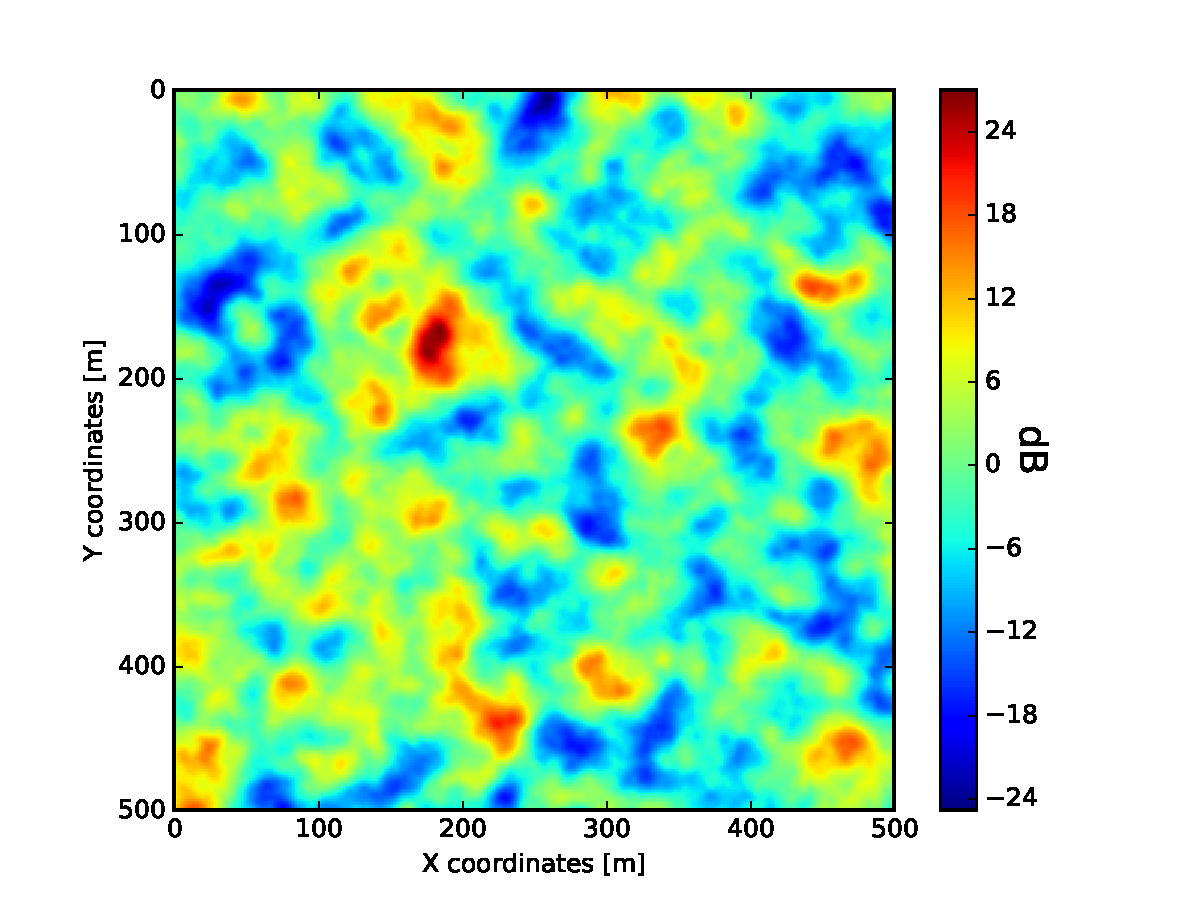
\includegraphics[width=1.1\linewidth]{figures/noise_after}
  \caption{Correlated Shadow Fading values}
  \label{fig:sf_correlated}
\end{subfigure}
\caption{Shadow Fading values before and after correlation adjustment}
\label{fig:SF}
\end{figure}


These shadow fading fading values are added to the pathloss values in order to fully account for all the obstacles in the way of the signal between two devices. The complete attenuation value then determines the received signal strength at the target device.

A summary of the relevant parameters utilized for the calculation of the pathloss can be seen in table \ref{tbl:PL}

\begin{table}[H]
\begin{center}
 \begin{tabular}{||p{7cm}|p{2.5cm}||} 
 \hline
 \textbf{Parameter} & \multicolumn{1}{|c||}{\textbf{Value}}\\
 \hline\hline
 Mean point density $\lambda$ & \multicolumn{1}{|c||}{$50 - 1000$} \\ 
 \hline
 Center Frequency $f_c$& \multicolumn{1}{|c||}{$2\,\text{GHz}$} \\
 \hline
 Wavelength $\lambda_{WL}$ & \multicolumn{1}{|c||}{$0.15\,\text{m}$}\\
 \hline
 Speed of light $c$ & \multicolumn{1}{|c||}{$3 \cdot 10^8\,\frac{\text{m}}{\text{s}}$}\\
 \hline
 Height of UE $h_{UE}$ & \multicolumn{1}{|c||}{$1.5\,\text{m}$} \\
 \hline
 Height of BS $h_{BS}$ & \multicolumn{1}{|c||}{$10\,\text{m}$} \\
 \hline
 Environment height $h_e$ & \multicolumn{1}{|c||}{$1\,\text{m}$} \\
 \hline
 Power decay constant $n_1$ & \multicolumn{1}{|c||}{$2.2$}\\
 \hline
 Power decay constant $n_2$ & \multicolumn{1}{|c||}{$4.0$}\\
 \hline
 Shadow Fading mean $\mu_{L_s}$ &\multicolumn{1}{|c||}{$0$} \\
 \hline
 Shadow Fading standard deviation $\sigma_{L_s}$ & \multicolumn{1}{|c||}{$7\,\text{dB}$}\\
 \hline
 Decorrelation distance $d_{corr}$ &\multicolumn{1}{|c||}{$8\,\text{m}$}\\
 \hline
\end{tabular}
\end{center}
\caption{Parameters relevant for pathloss calculation}
\label{tbl:PL}
\end{table}

\section{Random access procedure and interference} \label{RAP}
When reducing the load that the eNB experiences as a result of an increase in the amount of devices connecting to it by means of clustering, a large amount of the load is simply transferred to the cluster heads. These have then to take up the functions of the eNB in terms of implementing a random access procedure through which to service the UEs connecting to it. As mentioned in section \ref{B:D2D}, we contemplate an explicit separation of resources for normal BS to UE communication and D2D communication, putting further constraints on the ability of the cluster head to detect and separate signals using the same resource blocks. In order to best model these kinds of phenomena, the author utilized simulations developed by his supervisor, M.Sc. Mikhail Vilgelm, that were kindly put at his disposition for this work.

Firstly, a Poisson process is used in modeling the arrival of packages proceeding from connected UEs to the appropriate cluster head. This Poisson arrival process is analogous to that shown in equation \ref{eq:Poisson} and yields the amount of packages arrived at a certain point in time instead of points in an area. The arrival rate, $\lambda_A$ was set by recommendation of the author's supervisor to a level where the derivative of the throughput with respect to the arrival rate is positive, at $\lambda_A = 1.5$.

The requests are generated at the given rate and broadcast with a set transmission power $P_{Tx}$. Although there are many proposals for power control schemes in D2D communications, such as \cite{Erturk2013}, \cite{Wei2012} or \cite{Lee}, due to there being so many varied schemes and them adding such complexity to the simulation, it was decided that power control would not be part of the scope of this work. As in \cite{Klugel2014a}, we decide to use $P_{Tx} = 23\,\text{dBm}$ for our simulation, which is incidentally the power level used for coverage issue identification in \cite{3rdGenerationPartnershipProject;2012} and the maximum transmit power for public safety defined in \cite{3rdGenerationPartnershipProject;}, both by the 3GPP.

The power is then affected by the appropriate attenuation at the spot of the receiving device (see section \ref{PL}) and the resulting power is the received power $P_{Rx|dBm} = P_{Tx|dBm} - PL_{|dB}$. In order to assess whether a given signal has reached the cluster head with enough power to be detected, we look at the SINR (Signal-to-Interference-and-Noise-Ratio) of the transmission. For the calculation of the noise we use a thermal noise density $N_0 = -174\,\frac{\text{dBm}}{\text{Hz}}$, UE receiver noise figure $NF_{UE} = 9\,\text{dB}$ and system bandwidth $W = 10\,\text{MHz}$, as defined in \cite{3rdGenerationPartnershipProject;2012}. 

The incoming requests are checked for additional interference coming from other requests using the same preamble, both within and without the cluster. The received power $I$ of those interfering signals at the cluster head are added and that total added to the noise power $P_N$ to finally calculate the SINR, see equation \ref{eq:SINR}. As mentioned earlier, the available preambles for transmission of a D2D link are drawn from the overall pool of preambles available in LTE-A. As mentioned in \cite{Cox2012}, 64 preambles are available to the cell, only 6 of which are available for D2D communication. This is to allow normal cellular UEs to experience an acceptable QoS (Quality of Service), while still allowing other devices access to the network.

\begin{equation}\label{eq:SINR}
SINR = \frac {P_{Rx}} {I + P_N}
\end{equation}

As to the minimum SINR needed to connect to the cluster head, a threshold of $SINR_{thr} = 10\,\text{dB}$ was chosen within the range presented in \cite{3Gpp2009} for the minimum ratio necessary to transmit with ``an acceptably low BER (Bit Error Rate) in the output data.'' Those requests under the threshold will be filtered out before they are dealt with by the cluster head. Please note that although they are not counted towards successful requests, they will count towards interference values of other requests that may or may not clear the threshold.

Finally, requests clearing the threshold will be handled by the cluster head, who will then check for intra-cluster preamble collisions and give feedback, negative or positive, to the UEs. For simplicity's sake, feedback is assumed to arrive safely back at the UE; positive feedback elicits no action from the original transmitter. Upon reception of negative feedback, on the other hand, the UE ``backs off'' for an amount of time before attempting the connection once again at a later point in time. If the device is told to back off 20 times, it assumes the connection has failed completely and will not try again until another packet is generated at that UE. The time for each slot was set at $10\,\text{ms}$, while the overall simulation duration was put at $5\,\text{s}$.

Readers can find a summary of all used parameters for this stage on table \ref{tbl:RA}.

\begin{table}[H]
\begin{center}
 \begin{tabular}{||p{10cm}|p{2.5cm}||} 
 \hline
 \textbf{Parameter} & \multicolumn{1}{|c||}{\textbf{Value}}\\
 \hline\hline
 Request arrival rate $\lambda_A$ & \multicolumn{1}{|c||}{$1.5$} \\ 
 \hline
 Transmission power $P_{Tx}$& \multicolumn{1}{|c||}{$23\,\text{dBm}$} \\
 \hline
 Noise density $N_0$ & \multicolumn{1}{|c||}{$-174\,\frac{\text{dBm}}{\text{Hz}}$}\\
 \hline
 UE receiver noise figure $NF_{UE}$ & \multicolumn{1}{|c||}{$9\,\text{dB}$}\\
 \hline
 BS receiver noise figure $NF_{BS}$ & \multicolumn{1}{|c||}{$5\,\text{dB}$} \\
 \hline
 System Bandwidth $W$ & \multicolumn{1}{|c||}{$10\,\text{MHz}$} \\
 \hline
 Number of total LTE-A preambles & \multicolumn{1}{|c||}{$64$} \\
 \hline
 Number of preambles available for D2D communication& \multicolumn{1}{|c||}{$6$}\\
 \hline
 SINR threshold $SINR_{thr}$ & \multicolumn{1}{|c||}{$10\text{dB}$}\\
 \hline
 Slot duration & \multicolumn{1}{|c||}{$10\,\text{ms}$}\\
 \hline
 Total duration &\multicolumn{1}{|c||}{$5\,\text{s}$}\\
 \hline
\end{tabular}
\end{center}
\caption{Parameters relevant for random access and interference}
\label{tbl:RA}
\end{table}

The last piece of the puzzle is, of course, the actual mapping of UEs to cluster heads. These are fed into the random access and interference simulation by the clustering algorithms.

\section{Clustering Algorithms} \label{ClusteringAlgs}
Clustering algorithms determine which UEs will be connected to which cluster heads, as well as which UEs will turn into cluster heads in the first place. Because of the nature of our research (regarding D2D communication), we eschewed any schemes that required dedicated gateways into the networks. In the definition of the scope of this work, we also decided to leave out any algorithms with multi-hop possibilities, simply due to the sheer complexity that would have represented. Algorithms presented here thus feature only one aggregation stage at the cluster head, which then forwards the data to the eNB.

Most of the work done in clustering algorithms for wireless networks comes from the area of Wireless Sensor Networks (WSN), where large amounts of sensor nodes form a network communicating with a central unit of control. These types of structures lend themselves especially to grouping and aggregation, considering especially that there is often a lot of redundancy in the collected data. Energy efficiency and resilience of networks is often of paramount importance, in an attempt to minimize maintenance overhead. There have been several studies about clustering algorithms in this area, such as \cite{Jiang2009} or \cite{Afsar2014}. Looking toward WSNs seems like the closest logical step when considering D2D communications, but an effort was also made to look at algorithms not native to WSNs.

Additionally to WSN algorithms we included schemes normally used in statistical data analysis, specifically a couple of hierarchical clustering schemes. These often feature a progressive merging of clusters depending on a variety of criteria; distance is often used when determining the level of kinship two points or clusters possess. When possible, we have tried instead to use measures relevant to our research area, such as Signal-to-Noise Ratio (SNR) and Signal-to-Interference-and-Noise Ratio (SINR) to quantify connectivity. 

\subsection{LEACH} \label{LEACH}
One of the most influential clustering algorithms in WSNs is LEACH (Low-Energy Adaptive Clustering Hierarchy), presented in \cite{Heinzelman2000}. Despite its relative age, it promised ``localized coordination to enable scalability and robustness for dynamic networks'' and was designed to lower the amount of information transmitted to the base station. As can be seen in \cite{Afsar2014}, it has spawned many other algorithms based on its simple premises. 

LEACH works by randomly assigning its nodes as cluster heads according to a certain formula intended to yield a desired percentage $P_{LEACH}$ of CHs. Each node generates a uniformly distributed number between 0 and 1 and compares it to a threshold value $T(n)$. If the generated number is over that threshold it is designated to function as a cluster head.

Once cluster heads have been assigned for the whole of the network, an advertisement is broadcast, announcing to the other UEs which cluster heads are available. UEs then take the received signal strength as a proxy for distance and elect the nearest to their location. We simulate this behavior by creating a link to the received signal with the highest SNR. Signal must exceed an SNR of 0 to even be considered for a potential link, in order to ensure the advertisement is distinguishable from the noise. 

LEACH is designed to work with several rounds of CH assignment and data transfer in order to rotate the burden of CH selection, assuming a fixed set of nodes for a relatively long period of time. Seeing how our scenario is short-lived and features ideally mobile nodes, as well as a highly mutable network layout, we eschew the round structure. Consequently, the resulting  formula for the generation of the threshold value $T(n)$ can be seen in equation \ref{eq:LEACH}

\begin{equation}\label{eq:LEACH}
T(n) = \frac {P_{LEACH}}{1-P_{LEACH}\,(\text{mod}\,\frac {1}{P_{LEACH}})}
\end{equation}

Having observed just how many other clustering schemes it inspired, we decided to give LEACH particular importance in our testing, running simulations for it with a wider range of point densities $\lambda$, as well as more fine-grained data points.

\subsection{Complete-Link Clustering}
Also known as ``farthest neighbor clustering'', Complete-Linkage Clustering ``[t]ends to find compact clusters with equal diameters'' (\cite{Everitt2011}). It does so by defining the distance between two clusters as the maximum distance between their members, see equation \ref{eq:CLC}, from \cite{Shalizi2009}. 

\begin{equation}\label{eq:CLC}
d(A,B) = \min_{\vec{x} \in A,\,\vec{y} \in B} ||\vec{x}  - \vec{y}||
\end{equation}


Instead of using euclidean distance, as is the norm, we instead define the distance between two points as the SNR between them. Note that this ``reverses'' the algorithm's logic, meaning that instead of finding the minimum distance among all maximum distances in a cluster for a merge, we find the maximum SNR among all minimum SNRs inside a cluster. The algorithm then takes two clusters with the smallest such SNR ``distance'' and merges them.  Normally, it would continue to do so until there are no more clusters to merge, i.e. there only remains one cluster containing all the points in the set. In order to avoid this, with every potential merge of two clusters, we check if the potential D2D link is over a certain threshold. For this threshold we chose the same threshold introduced in section \ref{RAP}, $10 \text{dB}$. When no further links under that level are possible, the algorithms stops.

In this type of scheme, the election of the cluster head seems almost arbitrary. In order to maintain verisimilitude of the simulation, we designate the closest UE in terms of SNR to the eNB (position given in section \ref{mh_grid}) as the cluster head.


\subsection{Ward's Method}
Originally formulated as an approach in 1963, in \cite{Ward1963}, Ward's method provides an interesting cost metric for the merging of two clusters. As stated more succinctly in \cite{Shalizi2009}, the method ``says that the distance between two clusters, A and B, is how much the sum of squares will increase when we merge them''. Ward formulates a merging cost $\Delta(A,B)$ based on the the distance between the geographical center of each cluster and utilizes this information to merge the two clusters with the lowest cost:

\begin{equation}\label{eq:wards_cost}
\Delta(A,B) = \frac {n_A\,n_B}{n_A + n_B}\,||\vec{m_A} - \vec{m_B}||^2\,,
\end{equation}
with $n_A$ and $n_B$ the number of points in the cluster and $\vec{m_A}$ and $\vec{m_B}$ the center of clusters A and B. 

Here again, a limit must be provided for the algorithm not to form a single gigantic cluster; we continue using the D2D communication threshold $10 \text{dB}$. When the algorithm detects that there are no further connections possible over the given limit, it stops. A simple implementation of the algorithm can be observed in figure \ref{fig:ward_math}.

\begin{figure}[H]
\centering
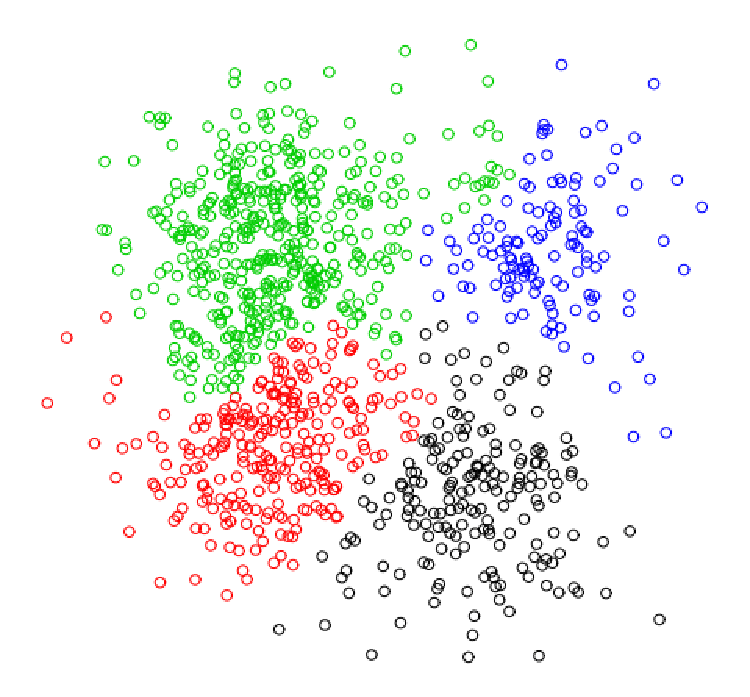
\includegraphics[width=.4\linewidth]{figures/ward_math}
\caption{Sample clustering as a result of Ward's Method \cite{Shalizi2009}}
\label{fig:ward_math}
\end{figure}

As with Complete-Link clustering, we assign a cluster head posterior to the creation of the cluster by designating the UE with the minimum SNR to the designated base station.
%  Conclusions (Zusammenfassung):
\chapter{Conclusions and Outlook}

In this thesis we sought to contribute to prospective solutions to problems well known in our field of study: as technology moves forward towards 5G, the Internet of Things and Smart Cities, the prospective explosion in the number of devices accessing wireless networks will place an inordinate burden on our existing infrastructure. We delved deeper into the use of D2D communications as a means to reuse the resources already available within LTE-A through cluster-centric data aggregation. Recognizing a gap in the evaluation of existing proposals, we intended to fairly compare and assess a handful of clustering schemes in their suitability to handle the types of scenarios which will be common in a not so distant future.

This work presents such a comparison within reason, despite some of its selected measures being less telling than was anticipated. It establishes a model that, while flawed in some aspects, deals with interference in the network, as well as the random access procedure of LTE-A, effectively and can be easily and readily expanded and amended to suit the future needs of investigation.

Our results show that Single-Linkage clustering with a predetermined number of target clusters outperforms most of its peers in all selected metrics and presents a very viable solution to the need to alleviate some of the pressure that the eNB will experience as a result of a high density of connecting devices. Despite being a very-well studied algorithm, it necessitates knowledge of the positions of all devices and presents a $O(n^2)$ computational complexity, which may pose a problem for time-constrained applications \cite{Everitt2011}. In this case, LEACH poses a very viable alternative, especially in higher densities of both UEs and CHs, where its behavior very closely resembles that of Single-Link clustering without the global knowledge or the complicated computations.

A big open question is of course, the decision to fix the arrival rate $\lambda_A$, as it hampered our tests and observations regarding interference. If the data being transferred is highly correlated and includes redundancy, as is often the case with WSNs, then lower request creation rate with higher number of devices makes sense: the frequency of the information that needs to be transmitted can afford to be lower. However, our simulation scenario was thought out to have very disparate data sources, making it intrinsically different from the WSN scenario. More research is needed with a $\lambda_A$ defined at the UE and not at the cluster head, to better evaluate the negative (and even potentially positive) effect that increased interference both within and without the cluster may cause. Thankfully this sort of adjustment seems relatively simple to make and integrate into the current models for future work. 

This leads us to the successful establishment of a simulation environment for evaluation of LTE-A and especially D2D, one of the main goals of this thesis. Despite much trial and error, the work presented here will, in the mind of the author, make a positive impact in his future investigative efforts, especially in the context of already ongoing studies in the institute.

The way for future work seems relatively clear. Firstly, the definition and implementation of an arrival rate that better reflects prospective traffic in a system with a growing number of connected devices to the cluster head is of paramount importance. In this way, the impact of interference in the studied systems can be understood more profoundly. Secondly, expanding the simulation into the traffic at the eNB, both from aggregated data and normal cellular traffic will better model the actual impact that D2D has on the reuse of the available pool of resources. Finally, the incorporation of other kinds of algorithms and schemes for aggregation, for instance multi-hop or power-controlling systems will expand the repertoire of mechanisms that we can evaluate.


% Appendix (Anhänge), could have multiple chaper-files:
\appendix
\chapter{}
The appendix may contain some listings of source code that has been used for simulations, extensive proofs or any other things that are strongly related to the thesis but not of immediate interest to the reader. 

% Abbreviations (Abkürzungsverzeichnis):
\chapter{Notation und Abkürzungen}
This chapter contains tables where all abbreviations and other notations like mathematical
placeholders used in the thesis are listed.
\begin{table}[h]
\begin{tabular}{ll}
AP & Access Point\\
BS & Base Station\\
CH & Cluster Head\\
CQI & Channel Quality Indicator\\
DCI & Downlink Control Information\\
D-SR & Dedicated Scheduling Request\\
D2D & device to device\\
eNodeB & evolved Node B or E-UTRAN Node B\\
FDD & Frequency Division Duplexing\\
H-ARQ & Hybrid-Automatic Repeat Request\\
IoT & Internet of Things\\
LOS & Line-of-Sight\\
LTE & Long Term Evolution\\
MCS & Modulation and Coding Scheme\\
METIS & Mobile and wireless communications Enablers for the Twenty-twenty Information Society \\
MTC & Machine Type Communication\\
NLOS & Non-Line-of-Sight\\
OFDM & Orthogonal Frequency Division Multiplexing\\
O2I & Outside-to-Inside\\
O2O & Outisde-to-Outside\\
PDCCH & Physical Downlink Control Channel\\
PDSCH & Physical Downlink Shared Channel\\
PPP & Poisson Point Process\\
PRB & Physical Resource Block\\
PUCCH & Physical Uplink Control Channel\\
PUSCH & Physical Uplink Shared Channel\\
RA & Random Access\\
RACH & Random Access Channel\\
SC-FDMA & Single Carrier Frequency Division Multiple Access\\
SR & Scheduling Request\\
SRS & Sounding Reference Signal\\
TDD & Time Division Duplexing\\
UE & User Equipment\\
WSN & Wireless Sensor Network\\
\end{tabular}
\end{table}


\listoffigures
\listoftables


% References (Literaturverzeichnis):
% a) Style (with numbers: use unsrt):
\bibliographystyle{alpha}
% b) The File:
\bibliography{biblio}


%%%%%%%%%%%%%%%%%%%%%%%%%%%%%%%%%%%%%%%%%%%%%%%%%%%%%%%%%%%%


%%%%%%%%%%%%%%%%%%%%%%%%%%%%%%%%%%%%%%%%%%%%%%%%%%%%%%%%%%%%


%%%%%%%%%%%%%%%%%%%%%%%%%%%%%%%%%%%%%%%%%%%%%%%%%%%%%%%%%%%%
\end{document}
